\documentclass[sigconf,nonacm]{acmart}


\settopmatter{printacmref=false}
\usepackage{needspace}
\usepackage{tabularx}
\renewcommand{\footnotetextcopyrightpermission}[1]{}

\acmYear{2026}
\acmISBN{}
\acmDOI{}

\title[Reproducing TinyTL for Few-Shot Learning]{Reproducing TinyTL and Exploring Few-Shot Adaptation Under Memory Constraints}
\subtitle{Group 4 -- Midterm Report}
\author{Tao Wang}
\email{twang209@jh.edu}
\affiliation{\institution{Johns Hopkins University}\city{Baltimore}\state{Maryland}\country{USA}}
\author{Yujia Zhang}
\email{yzhan876@jh.edu}
\affiliation{\institution{Johns Hopkins University}\city{Baltimore}\state{Maryland}\country{USA}}
\author{Chen Chen}
\email{cchen320@jh.edu}
\affiliation{\institution{Johns Hopkins University}\city{Baltimore}\state{Maryland}\country{USA}}
\renewcommand{\shortauthors}{Wang, Zhang, and Chen}

\begin{document}
\begin{abstract}
On-device training is limited by memory and labeled data. TinyTL reduces training memory by freezing pretrained weights, but how it should be configured with only a few images per class is unclear. We reproduce TinyTL, evaluate it at 2, 5, and 10 shots on Flowers102 and FGVC-Aircraft, and test low-cost changes to adaptation depth, block selection, classifier initialization, and batch size. Training only the later blocks, a configuration we call T4, reduces measured GPU peak memory from 557 to 105\,MiB, a reduction of 81\%, while staying within 1 percentage point of full TinyTL on Flowers at all three shot counts and Aircraft at 2--5 shots. On Aircraft at 10 shots, however, it loses 3.35 percentage points. Class-mean imprinting improves T4 accuracy by 0.56--1.46 percentage points at 2 and 5 shots but not at 10 shots, while our Fisher-based choices among truncation points and among individual blocks do not beat fixed truncation. Batch size 1 shows no severe accuracy collapse on Aircraft at 5 and 10 shots and recovers the loss of truncation at 10 shots, but trains about five times more slowly under a similar memory budget. These results support simple, task-dependent configurations rather than a single choice for every setting.
\end{abstract}

\keywords{TinyTL, few-shot learning, on-device training, memory-efficient adaptation}
\maketitle

\section{Introduction}
IoT devices may need to adapt pretrained models to local data without sending private examples to a server. However, on-device training is harder than inference: backpropagation stores intermediate activations, and users may have only a few labeled images. Both training memory and data availability constrain adaptation.

Tiny Transfer Learning, or TinyTL, freezes pretrained weights and updates biases and lightweight residual modules to reduce memory \cite{cai2020tinytl}. It was mainly evaluated with full training sets, leaving open how much adaptation is needed with only a few examples per class. TinyTrain instead studies task-aware updates under data scarcity, but uses a more complex meta-training pipeline \cite{kwon2024tinytrain}. The papers also report different small-batch behavior for TinyTL under different experimental setups. We therefore ask: \emph{How should TinyTL be configured to balance accuracy, memory, and computation when labeled data are scarce?}

We first reproduce TinyTL, then test shorter backward paths and TinyTrain-inspired rules for choosing where to truncate and which blocks to update. Separately, we test class-mean imprinting as a simple classifier initialization without meta-training, and compare smaller batches with shorter backward paths. Our main finding is that late-block adaptation is often sufficient, but Aircraft at 10 shots needs more depth or a smaller batch. We also report negative results for both Fisher selection rules and identify the remaining cases that require testing.

\section{Related Work}
\textbf{Memory-efficient training.} TinyTL shows that saving activations for gradients can be more costly than storing trainable parameters. It freezes convolution weights while training biases and lite residual modules; at 224-pixel input, its Flowers102 experiment reports 95.5\% accuracy and a 37\,MB profiler estimate, compared with 391\,MB for full fine-tuning \cite{cai2020tinytl}. Lin et al. combine quantization-aware scaling, sparse updates, and a specialized engine for extremely memory-constrained training \cite{lin2022ondevice}. Unlike that work, we keep the released TinyTL architecture and training framework and vary which parts require backward computation.

\textbf{Few-shot adaptation.} TinyTrain uses meta-learning and task-aware selection of layers and channels; it finds that useful layers often lie toward the end of the network, motivating our truncation experiments \cite{kwon2024tinytrain}. TinyTrain also reports that its TinyTL baseline performs better than last-layer-only training, but degrades at small batch sizes. TinyTL reports little small-batch degradation with GroupNorm \cite{cai2020tinytl,wu2018groupnorm}. Because the protocols differ, we test batch size directly rather than assuming either result generalizes. Related parameter-selection work includes p-Meta, which meta-learns which layers and channels to update \cite{qu2022pmeta}. Weight imprinting provides another idea: initializing a classifier using normalized features of labeled examples \cite{qi2018imprinted}. We use an unnormalized variant of this idea as a low-cost addition to TinyTL, not as a reproduction of TinyTrain's meta-learning method.

\begin{figure*}[!t]
  \centering
  \includegraphics[width=0.86\textwidth]{fig3_configurations.pdf}
  \caption{LB and four shorter-backward-path configurations. Every configuration retains all forward features; ``trained'' means that biases, lite residuals, or classifier parameters receive gradients. Memory values are measured GPU peaks at batch size 8.}
  \Description{A matrix comparing LB, T2, T3, T4, and last by trainable stages and GPU memory. All configurations use the full forward model.}
  \label{fig:configs}
\end{figure*}

\section{Research Questions and Approach}
We focus on three questions. \textbf{RQ1:} How does TinyTL perform with few labeled examples, and how much adaptation is needed across tasks and shot counts? \textbf{RQ2:} Can a TinyTrain-inspired choice of truncation point or blocks, or class-mean imprinting, improve the accuracy--memory--compute trade-off at low cost? \textbf{RQ3:} Under a limited memory budget, is reducing batch size or shortening the backward path more effective?

Our reference, \textbf{LB}, is full TinyTL-L+B: all biases, lite residuals, and the classifier are trainable. \textbf{T2}, \textbf{T3}, and \textbf{T4} start updating at blocks 9, 13, and 17, so they update stages 2--5, 3--5, and 4--5; \textbf{last} trains only the classifier, as shown in Fig.~\ref{fig:configs}. All five configurations run the \emph{same forward network}, including every lite residual. They differ only in trainable parameters and the length of the backward path. For block selection, we also use block sets that update only the chosen blocks and the classifier: \textbf{C} updates blocks 16--21, and \textbf{FS} updates blocks 15, 16, 17, and 19.



\begin{figure}[!t]
  \centering
  \includegraphics[width=\columnwidth]{fig2_memory_vs_accuracy.pdf}
  \caption{Accuracy difference versus measured peak GPU memory at $k=5$. T4 stays close to LB with much lower memory. Hollow T2 markers denote exploratory comparisons.}
  \Description{For both Flowers102 and Aircraft at five shots, the T4 configuration is close in accuracy to LB while using much less GPU memory; last loses substantial accuracy.}
  \label{fig:memory}
\end{figure}

\begin{figure*}[!t]
  \centering
  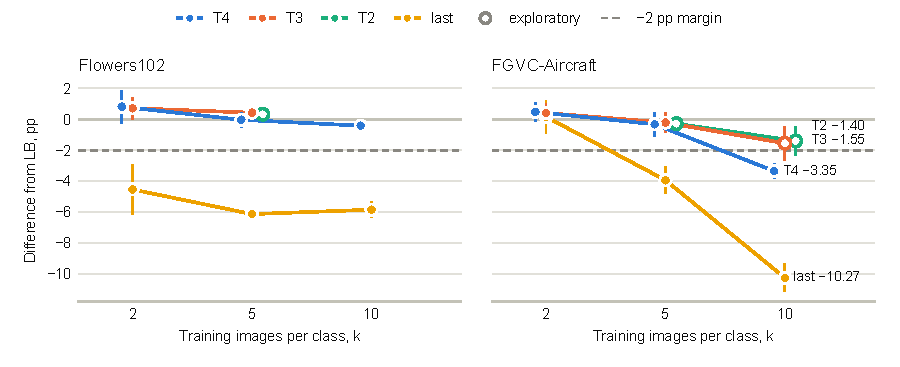
\includegraphics[width=0.85\textwidth]{fig1_k_vs_accuracy.pdf}
  \caption{Accuracy relative to LB at 2, 5, and 10 training images per class, with 93\% intervals. The dashed line marks $-2$\,pp; hollow markers denote exploratory comparisons. The plotted differences alone do not establish non-inferiority.}
  \Description{For Flowers102 T4 remains within one percentage point of LB from two to ten shots. For Aircraft T4 falls further behind at ten shots.}
  \label{fig:shots}
\end{figure*}


\section{Experimental Design}
\textbf{Shared setup.} We use ProxylessNAS-Mobile \cite{cai2019proxylessnas} with TinyTL's released lite-residual weights, which use weight standardization and GroupNorm \cite{qiao2019ws,wu2018groupnorm}, 224-pixel inputs, and 8-bit quantization of frozen weights. Training uses Adam, cosine learning-rate decay, 50 epochs, label smoothing 0.7, and batch size 8 unless stated otherwise. We evaluate the final-epoch checkpoint rather than selecting one by validation accuracy. Learning rates are fixed after the $k=5$ pilot and reused across shot counts; imprinting uses the rates selected for random initialization, and block sets use the T4 rate. Flowers102 has 102 classes \cite{nilsback2008flowers}; FGVC-Aircraft has 100 aircraft models \cite{maji2013aircraft}. In this setup, Flowers is the closer transfer task and Aircraft the more distant one. We draw $k\in\{2,5,10\}$ labeled images per class from the training split and evaluate on the test split, which has 6,149 Flowers102 and 3,333 Aircraft images. Because the Flowers training split has 10 images per class, $k=10$ on Flowers uses all of it.

\textbf{Fair comparisons.} Runs are paired by random seed: configurations share sampled images, classifier initialization, quantized weights, and data order. The main $k=5$ depth study uses up to 10 paired seeds for Flowers and six for Aircraft; some arms use five. Added shot-count, imprinting, batch, and block-selection experiments use five paired seeds. We report test-accuracy differences $d=A_{\mathrm{cfg}}-A_{\mathrm{LB}}$ in percentage points, abbreviated pp, where $A_{\mathrm{cfg}}$ is the accuracy of the configuration being tested. The protocol uses a 2-pp non-inferiority margin: \emph{retains} means evidence that the mean loss relative to LB is less than 2\,pp, not that the methods are identical. Two-sided 93\% paired $t$ intervals correspond to a one-sided level of 0.035 before multiplicity correction. The reported intervals are unadjusted; retention decisions for the prespecified comparisons of T3, T4, and \emph{last} with LB use Holm-corrected tests. T2 and later added comparisons, including T3 at $k=10$, are exploratory. Peak GPU memory and step time are measured on an RTX 3060, not an IoT device, and backward MACs are counted from the network definition.

\textbf{Experiment overview.} The following table summarizes what has been tested; not every configuration was tested at every shot count.

\begin{center}
  \footnotesize
  \renewcommand{\arraystretch}{1.15}
  \begin{tabularx}{\columnwidth}{@{}lX@{}}
    \toprule
    Study & Scope and current status \\
    \midrule
    E0 & Full-data Flowers102 reproduction and GPU memory measurement completed. \\
    E1 & RQ1. Both datasets, $k=5$, all five backward-depth choices completed. \\
    E2 & RQ1. Both datasets, $k=2,10$, selected depths completed, including Aircraft $k=10$ T3 and T2. \\
    E3 & RQ2. Fisher selection among truncation points at $k=5$ and among individual blocks on Aircraft $k=10$ and Flowers $k=5$ completed. \\
    E4 & RQ2. Imprinting tested for T4, \emph{last}, and LB at $k=2,5$ and for T4 at $k=10$. \\
    E5 & RQ3. Batch-size comparison completed for Aircraft $k=5$ and $k=10$; Flowers planned. \\
    E6 & Learning-rate, epoch-budget, and checkpoint checks completed. \\
    \bottomrule
  \end{tabularx}
\end{center}

\textbf{Two low-cost methods.} For E3, we estimate TinyTrain's Fisher importance \cite{kwon2024tinytrain} from a few labeled samples for three groups of stages, namely stage 2, stage 3, and stages 4--5, normalize scores by parameter and backward-compute cost, and use a prefix-greedy rule to choose a feasible \emph{contiguous} truncation point. The rule is compared with the deepest fixed configuration that fits the same memory budget. We then apply the same importance to individual blocks: each of the 19 lite-residual blocks is scored, normalized by its parameter count and its marginal measured memory, and added in order of score whenever the measured peak of the selected set stays within 128\,MiB. This non-contiguous selection is compared with T4 and with C, the deepest contiguous truncation at block granularity within the same budget. For E4, we average pretrained features $\mu_c$ of each class and initialize its classifier weight and bias as $w_c=2\mu_c/\tau$ and $b_c=-\lVert\mu_c\rVert^2/\tau$, with a temperature $\tau$ chosen from the training loss. Unlike the original imprinting method, we do not normalize the features. We then fine-tune normally and compare with random classifier initialization on the same samples.





\section{Preliminary Results}
\subsection{Reproduction and adaptation depth: E0--E2}
Our full-data Flowers102 reproduction reaches \textbf{95.20\%} top-1 accuracy, close to TinyTL's 95.5\%. At batch size 8, the LB profiler estimates 37.1\,MB while PyTorch measures a peak of \textbf{557.2\,MiB}; an idealized implementation lower bound is 246\,MiB. These estimates account for memory differently. In our implementation, saved GroupNorm inputs alone use about 172--175\,MiB. We therefore use \emph{measured PyTorch peak memory} for all configuration comparisons.

At $k=5$, LB reaches 85.03\% on Flowers and 25.74\% on Aircraft. T4 differs from LB by only $-0.03$ and $-0.32$\,pp, respectively; both pass the prespecified retention tests. Meanwhile, T4 uses \textbf{105.2\,MiB}, 81\% less than LB's 557.2\,MiB, and reduces backward computation from 459\,M to 125\,M MACs per image. The classifier-only \emph{last} configuration loses 6.14\,pp on Flowers and 3.94\,pp on Aircraft. Figure~\ref{fig:memory} shows the depth--memory--accuracy trade-off.



The number of examples changes both baseline accuracy and the required adaptation. From $k=2$ to 10, LB improves from 68.1\% to 92.0\% on Flowers and from 13.9\% to 39.5\% on Aircraft. T4 stays within 1\,pp of LB at every tested $k$ on Flowers and at $k=2,5$ on Aircraft. At $k=10$ on Aircraft, however, T4 loses \textbf{3.35\,pp}. Increasing backward depth to T3 reduces that loss to 1.55\,pp, but its interval $[-2.58,-0.51]$ crosses the 2-pp margin, so retention remains unresolved. T2 reduces the loss only slightly further, to 1.40\,pp with interval $[-2.28,-0.52]$, while using 58\,MiB more memory than T3. Figure~\ref{fig:shots} shows these differences; the T3 and T2 comparisons at $k=10$ are exploratory. With fixed 50-epoch training, $k=2$ also has fewer optimizer steps; a one-seed longer run suggests this affects accuracy, so the observed pattern may not be caused by sample count alone.



\begin{figure}[!t]
  \centering
  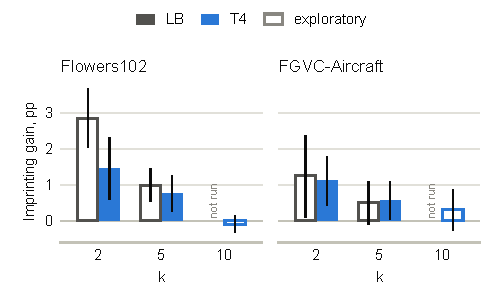
\includegraphics[width=0.94\columnwidth]{fig4_imprinting_gain.pdf}
  \caption{Gain from class-mean imprinting over random classifier initialization after 50 epochs, with 93\% intervals. Hollow bars denote exploratory comparisons; LB was not run at $k=10$.}
  \Description{Bar chart of imprinting gains for LB and T4 on Flowers102 and Aircraft. Gains are positive at two and five shots and near zero for T4 at ten shots.}
  \label{fig:imprint}
\end{figure}

\subsection{Fisher selection and imprinting: E3--E4}
At 128\,MiB, the Fisher prefix-greedy rule selects \emph{last} for all tested seeds, although T4 also fits. The rule admits only prefixes of the importance ranking: it does not skip an infeasible higher-ranked group to choose lower-ranked groups. The top-ranked early-stage group exceeds the budget, leaving only the classifier. This exposes a limitation of this restricted rule. We measure \emph{regret} as the accuracy of the best feasible configuration for each seed minus the accuracy of the chosen one. Fisher has mean regret of 5.90\,pp on Flowers and 3.44\,pp on Aircraft, versus zero for the deepest feasible fixed T4 rule in this comparison. At 256\,MiB, both Fisher and the fixed rule choose T2. This negative result applies to \emph{selection among truncation points}, so we also tested the selection of individual blocks.

Selecting individual blocks saves less memory than expected. Gradients must still flow back through every block after the earliest selected one, so updating a block alone saves only 2--10\% of memory compared with updating it and every later block. Under 128\,MiB, C updates blocks 16--21 and uses 119.2\,MiB, while skipping blocks lets the rule reach block 15. On all five seeds of both Aircraft at $k=10$ and Flowers at $k=5$, the rule selected the same set, FS, which uses 127.1\,MiB, so in practice the selection did not depend on the task. FS does not beat T4: the difference is $+0.06$\,pp on Aircraft with interval $[-0.41,0.53]$ and $-1.15$\,pp on Flowers with interval $[-1.38,-0.93]$. FS is also 1.15 and 1.69\,pp below C, and adding imprinting to both FS and T4 does not change these conclusions. In a post-hoc comparison, C exceeds T4 by 1.21\,pp on Aircraft and 0.54\,pp on Flowers with 14\,MiB more memory, which suggests that truncation granularity matters more than task-aware selection. Table~\ref{tab:budget} summarizes the configurations within 128\,MiB.

\begin{table}[!t]
  \caption{Configurations within a 128\,MiB training-memory budget at batch size 8 unless noted. Entries are paired differences from LB at batch size 8 in pp, shown as $d\pm$ the half-width of the 93\% interval over seeds 0--4. Flowers values therefore differ slightly from the 10-seed results above.}
  \label{tab:budget}
  \footnotesize
  \setlength{\tabcolsep}{4pt}
  \begin{tabular}{@{}lrrr@{}}
    \toprule
    Configuration & MiB & Aircraft $k=10$ & Flowers $k=5$ \\
    \midrule
    LB accuracy & 557.2 & 39.47\% & 84.83\% \\
    \midrule
    T4 & 105.2 & $-3.35\pm0.40$ & $-0.19\pm0.59$ \\
    T4 with imprinting & 105.2 & $-3.04\pm0.34$ & $+0.57\pm0.59$ \\
    FS, blocks 15--17 and 19 & 127.1 & $-3.29\pm0.69$ & $-1.35\pm0.47$ \\
    C, blocks 16--21 & 119.2 & $-2.15\pm0.57$ & $+0.35\pm0.64$ \\
    LB at batch size 1 & 122.1 & $+0.07\pm2.32$ & -- \\
    \emph{last} & 67.4 & $-10.27\pm0.85$ & $-6.09\pm0.49$ \\
    \bottomrule
  \end{tabular}
\end{table}

Class-mean imprinting improves T4 after 50 epochs by \textbf{1.46} and \textbf{0.76}\,pp on Flowers and \textbf{1.12} and \textbf{0.56}\,pp on Aircraft, at $k=2$ and $k=5$, respectively, as shown in Fig.~\ref{fig:imprint}. LB benefits as well, by 2.85 and 0.99\,pp on Flowers and 1.25 and 0.50\,pp on Aircraft, although the Aircraft gain at $k=5$ is not significant; with imprinting applied to both, T4 stays within 0.6\,pp of LB. At $k=10$, the gain disappears: imprinting changes T4 by $-0.09$\,pp on Flowers and $+0.32$\,pp on Aircraft, and T4 with imprinting still loses 3.04\,pp to LB on Aircraft. At $k=5$, T4 with imprinting trained for only 10 epochs is 0.92\,pp below 50-epoch LB on Flowers, using about 0.12 times its estimated training computation; the Aircraft gap is 2.42\,pp. These LB, $k=10$, and short-run results are exploratory.



\Needspace{8\baselineskip}
\subsection{Batch size and robustness: E5--E6}
For Aircraft at $k=5$, LB at batch size 1 uses 122.1\,MiB versus 557.2\,MiB at batch size 8. Accuracy changes by $-1.04$\,pp with a 93\% interval of $[-3.31,1.22]$: there is no observed five-point average collapse, but the interval does not establish retention within 2\,pp. Under the \emph{same 128\,MiB budget}, LB-b1 versus T4-b8 has a paired difference of $-0.55$\,pp with interval $[-2.91,1.81]$, so the accuracy comparison remains uncertain. T4-b8 uses slightly less memory, 105.2 versus 122.1\,MiB, and takes 8 rather than 34 minutes per run. At $k=10$, where T4 loses accuracy, LB-b1 changes accuracy by $+0.07$\,pp relative to LB-b8 and exceeds T4-b8 by 3.42\,pp with interval $[0.84,6.00]$, but its results vary more across seeds and each run takes 64 rather than 12 minutes. E6 learning-rate and training-duration checks do not reverse the main depth result.

\balance
\section{Proposed Experiments and Expected Outcomes}
\textbf{Complete the depth study for RQ1.} We will add paired seeds to T3, because T4 loses 3.35\,pp on Aircraft at $k=10$ and the intervals of T3 and T2 cross our margin. We expect deeper adaptation to keep the mean loss below 2\,pp, but the additional seeds are needed before a firm retention conclusion.

\textbf{Confirm block-level truncation for RQ2.} C exceeded T4 only in a post-hoc comparison. We will test C on Aircraft at $k=5$ and Flowers at $k=10$, and with imprinting on Aircraft at $k=10$ and Flowers at $k=5$. We expect C to match or slightly exceed T4; if it does not, we will keep stage-level truncation.

\textbf{Test small batches further for RQ3.} We will repeat the batch-size check on Flowers at $k=5$ and compare newly initialized lite residuals to the released pretrained ones at batch sizes 1 and 8. We expect batch size 1 not to collapse on Flowers either. Comparing module initializations may help explain the papers' different observations. Finally, we will combine all results into configuration guidance by task, shot count, and memory budget.

\section{Discussion and Limitations}
Our current practical starting point is \textbf{T4 at batch size 8}, with class-mean imprinting at $k=2,5$ on both datasets. It substantially reduces memory while staying close to LB in those settings. It is \emph{not} a universal recommendation: Aircraft at $k=10$ needs deeper adaptation, and within 128\,MiB either LB at batch size 1 or the block-level truncation C is preferable there; imprinting does not help at $k=10$. Neither Fisher rule has improved over fixed truncation.

Our conclusions are limited to one backbone, 224-pixel images, and two datasets. Some supplemental comparisons use five seeds and follow the initial observations. Fixed epoch counts mean different shot counts receive different numbers of optimizer steps, and learning rates were not tuned separately for every $k$. The block-selection rule chose the same blocks for every seed and both datasets, so it does not test truly task-dependent selection. Memory and time come from a PyTorch RTX 3060 setup, so they do not establish IoT-device RAM, energy, or speed. The final experiments will test how far the current configuration guidance generalizes.

\bibliographystyle{ACM-Reference-Format}
\bibliography{references}
\end{document}
